\documentclass[9pt,twocolumn,twoside,]{pnas-new}

% Use the lineno option to display guide line numbers if required.
% Note that the use of elements such as single-column equations
% may affect the guide line number alignment.


\usepackage[T1]{fontenc}
\usepackage[utf8]{inputenc}

% tightlist command for lists without linebreak
\providecommand{\tightlist}{%
  \setlength{\itemsep}{0pt}\setlength{\parskip}{0pt}}


% Pandoc citation processing
\newlength{\cslhangindent}
\setlength{\cslhangindent}{1.5em}
\newlength{\csllabelwidth}
\setlength{\csllabelwidth}{3em}
\newlength{\cslentryspacingunit} % times entry-spacing
\setlength{\cslentryspacingunit}{\parskip}
% for Pandoc 2.8 to 2.10.1
\newenvironment{cslreferences}%
  {}%
  {\par}
% For Pandoc 2.11+
\newenvironment{CSLReferences}[2] % #1 hanging-ident, #2 entry spacing
 {% don't indent paragraphs
  \setlength{\parindent}{0pt}
  % turn on hanging indent if param 1 is 1
  \ifodd #1
  \let\oldpar\par
  \def\par{\hangindent=\cslhangindent\oldpar}
  \fi
  % set entry spacing
  \setlength{\parskip}{#2\cslentryspacingunit}
 }%
 {}
\usepackage{calc}
\newcommand{\CSLBlock}[1]{#1\hfill\break}
\newcommand{\CSLLeftMargin}[1]{\parbox[t]{\csllabelwidth}{#1}}
\newcommand{\CSLRightInline}[1]{\parbox[t]{\linewidth - \csllabelwidth}{#1}\break}
\newcommand{\CSLIndent}[1]{\hspace{\cslhangindent}#1}


\templatetype{pnasresearcharticle}  % Choose template

\title{Problème universelle de reproductibilité en science et une piste
de solution}

\author[a]{Édouard Nadon-Beaumier}

  \affil[a]{Université de Sherbrooke, Départment de biologie, 2500
Boulevard de l'Université, Sherbrooke, Québec, G1V 0A9}


% Please give the surname of the lead author for the running footer
\leadauthor{}

% Please add here a significance statement to explain the relevance of your work
\significancestatement{}


\authorcontributions{}



\correspondingauthor{\textsuperscript{} }

% Keywords are not mandatory, but authors are strongly encouraged to provide them. If provided, please include two to five keywords, separated by the pipe symbol, e.g:


\begin{abstract}
Avec l'augmentation des prépublications scientifique dues à la pandémie
mondiale de SRAS-CoV-2 plusieurs problématiques des domaines
scientifiques font couler de l'encre et animent les sujets de
conversation. La perte de confiance d'une partie de la population
démontre l'incapacité de la science à produire des résultats avec une
transparence et une reproductibilité suffisamment grande. Une réforme du
système de publication par la réduction de la pression à publier, un
changement d'emphase de publications de résultats positive, une
amélioration de l'intégrité scientifique et réduire l'importance d'une
seule équipe sont nécessaires pour redonner confiance et améliorer les
connaissances scientifiques.
\end{abstract}

\dates{This manuscript was compiled on \today}
\doi{\url{www.pnas.org/cgi/doi/10.1073/pnas.XXXXXXXXXX}}

\begin{document}

% Optional adjustment to line up main text (after abstract) of first page with line numbers, when using both lineno and twocolumn options.
% You should only change this length when you've finalised the article contents.
\verticaladjustment{-2pt}



\maketitle
\thispagestyle{firststyle}
\ifthenelse{\boolean{shortarticle}}{\ifthenelse{\boolean{singlecolumn}}{\abscontentformatted}{\abscontent}}{}

% If your first paragraph (i.e. with the \dropcap) contains a list environment (quote, quotation, theorem, definition, enumerate, itemize...), the line after the list may have some extra indentation. If this is the case, add \parshape=0 to the end of the list environment.

\acknow{}

\hypertarget{introduction}{%
\section{Introduction}\label{introduction}}

Avec l'effet de la pandémie de SRAS-CoV-2 et ses variants, plusieurs
problèmes du domaine de la science on fait surface. Une des
problématiques a été le besoin en connaissance sur ce virus et la
quantité phénoménale d'articles publiés dans des journaux qui ont été
par la suite retirer par la suite pour de multiple raison comme
l'intégrité scientifique (1). Ceci à causer dans certains cas de la
désinformation dans les connaissances scientifiques et nous avons eu la
possibilité d'observer un bris de confiance entre certaines personnes du
public et la science avec plusieurs mouvements de protestations contre
la vaccination de la Covid-19. De façon plus générale, le manque de
transparence et de standard dans la production de réplication dans le
jeu de données des recherches publiés cause un manque de confiance dans
les résultats obtenus par les différents chercheurs et leur équipe. Dans
une étude avec 1576 chercheurs dans différents domaines de la science,
52\% d'eux sont d'accord qu'il y a une crise sur la reproductibilité des
recherches produites. De plus, 73\% des répondants affirment qu'au moins
50\% des résultats obtenus sont véritables (2). Il est utopique de
s'attendre à avoir une confiance de 100\% pour toutes les recherches
publiées surtout en science lorsque les chercheurs travaillent avec des
probabilités. Toutefois, le pourcentage de confiance minimum devrait
être plus élevée que la moitié des publications. Il est impératif pour
l'avancement des bonnes connaissances scientifiques et pour regagner la
confiance de certaines parties du public d'améliorer la reproductibilité
et la transparence des publications des différents domaines. Un
changement dans la mentalité de publication est nécessaire par une
diminution de la pression et de la quantité qu'un scientifique doit
publier, par la diminution de l'emphase mise sur des articles à
résultats positifs, par l'augmentation de la transparence des jeux de
données utilisées.

\hypertarget{emphase-des-articles-publications}{%
\section{Emphase des articles
publications}\label{emphase-des-articles-publications}}

Les journaux les plus reconnus dans le monde scientifique reçoivent
quotidiennement plus d'articles que ce qu'ils peuvent publier. Ainsi,
les articles qui sont publiés doivent donner des résultats positifs à
leur supposition de base et qui sont frappants afin d'attirer
l'attention des lecteurs. Ceci crée une culture d'hypercompétition pour
la publication des articles ce qui incite les chercheurs à obtenir des
conclusions en faveur de leur hypothèse afin d'augmenter leurs chances
d'être publié par ces journaux prestigieux (3). Toutefois, cette
incitative à avoir uniquement des résultats positifs selon le modèle
d'analyse de Grime et ses associés en 2018 diminue la fiabilité des
résultats et augmente la proportion d'utilisation de faux positif dans
le jeu de données afin d'obtenir des conclusions. Cette fraude par la
manipulation de données permet aux auteurs d'améliorer leur chance de
publication et d'obtenir de futures subventions au détriment d'un
travail scientifique rigoureux et l'avancer des connaissances fiables.
Cette problématique pourrait être réglée par un mouvement des journaux
vers une acceptation accru des articles démontrant une excellente
rigueur scientifique comme le fait le journal PLoS ONE. Depuis, 2017
d'autres journaux comme Royal Society Open Science et Nature Scientific
Reports on fait le changement mais l'implication des grands journaux
comme Nature, Cell, Cancer Journal for Clinicians auraient un impact
encore plus significatif sur le changement de mentalité du domaine
scientifique sur le type de publication priorisé (4)

\hypertarget{pression-de-publication}{%
\section{Pression de Publication}\label{pression-de-publication}}

Le mantra ``publier ou périr'' est couramment utilisé en science
principalement dans les domaines médicaux car plusieurs évaluateurs
académiques favorisent les publications scientifiques où bon sain
apporter aux patients par un clinicien. Ceci est une récompense sous
forme monétaire et de prestige des individus ayant un grand nombre de
publication et aux nombres de citations de leurs articles (5). Ainsi, un
scientifique aspirant à un meilleur poste doit fournir des résultats
constants et rapides afin de pouvoir publier et rester à jour avec un
domaine de grande concurrence pour les sources de financement
insuffisantes pour tous les chercheurs (6). L'obtention d'opportunité
d'emploi et d'avancement de carrière devrait favoriser la qualité des
travaux publiés et de l'intégrité éthique et scientifique de la personne
plutôt que son nombre de publications et de citations. Une solution à se
produire est de réduire la quantité de productivité par auteur et tenter
d'atteindre l'équilibre optimal en matière de productibilité
scientifiques et de la qualité au travers la réplication et la
transparence de la méthode utilisée et de tous les résultats obtenus (3)

\begin{figure}
\centering
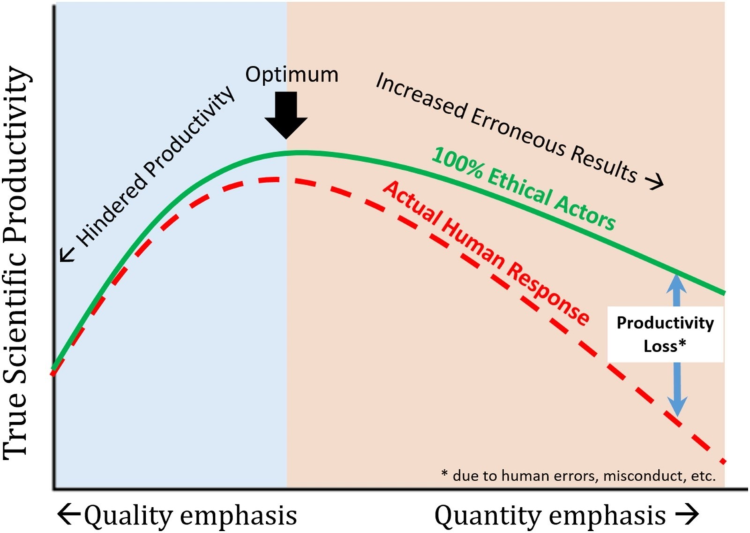
\includegraphics[width=0.5\textwidth,height=0.4\textheight]{"../Article_de_Edouard/image.pdf"}
\caption{Modélisation de la production d'articles en science.
\label{fig:plot1}}
\end{figure}

Avec une productibilité plus faible et une meilleure qualité de
publication, la reproductibilité des expériences et des résultats
obtenus seraient améliorées. Pour atteindre cette réduction de pression
de publication, le domaine scientifique doit retirer du moins réduire la
quantité d'importance octroyée à la quantité de publication vers des
publications avec un haut taux de reproductibilité et des analyses
pertinentes avec une puissante statistique élevée.

\hypertarget{piste-de-solution-uxe0-la-reproductibilituxe9}{%
\section{Piste de solution à la
reproductibilité}\label{piste-de-solution-uxe0-la-reproductibilituxe9}}

Une option due qui peut être mal vue est la diminution de l'importance
humaine dans le projet avec l'utilisation de la technologie afin de
réduire les erreurs humaines et garder une vision pragmatique dans
toutes les étapes de la recherche scientifique. Cette solution
potentielle peut être difficile d'implémenter en réalité. Une façon
rapide et efficace de viser une meilleure reproductibilité est
d'améliorer l'évaluation de la littérature scientifique actuelle. Ceci
requiert que les scientifiques passent plus de temps dans la lecture
scientifique, du temps qui est perdu dans les laboratoires et qui est
mal vue avec la science moderne de production d'articles le plus
rapidement possible (7). Plusieurs équipes de recherche travaillent sur
les mêmes sujets ou des sujets similaires. En diminuant l'importance de
la première donnée à la première équipe qui publie des résultats, ils
frauderaient mettre la même importance pour toutes les recherches
connexes (8). Les résultats des autres équipes pourraient réduire
l'effet de biais et confirmer la viridité des analyses des différentes
équipes. En somme, le problème de reproductibilité n'est pas un nouveau
sujet dans le domaine et plus longtemps le problème reste non régler
plus il sera difficile de le résoudre. Pour la résolution toutes
personnes impliquées dans le domaine scientifique devront jouer un rôle
pour viser une meilleure reproductibilité.

\pnasbreak

\hypertarget{refs}{}
\begin{CSLReferences}{0}{0}
\leavevmode\vadjust pre{\hypertarget{ref-khalifa2021fast}{}}%
\CSLLeftMargin{1. }
\CSLRightInline{Khalifa AA, Ahmed AM (2021) How fast is the peer-review
process for orthopaedic publications related to the covid-19 pandemic?
\emph{Journal of clinical orthopaedics and trauma} 12(1):9--15.}

\leavevmode\vadjust pre{\hypertarget{ref-baker20161}{}}%
\CSLLeftMargin{2. }
\CSLRightInline{Baker M (2016) 1,500 scientists lift the lid on
reproducibility. \emph{Nature} 533(7604).}

\leavevmode\vadjust pre{\hypertarget{ref-edwards2017academic}{}}%
\CSLLeftMargin{3. }
\CSLRightInline{Edwards MA, Roy S (2017) Academic research in the 21st
century: Maintaining scientific integrity in a climate of perverse
incentives and hypercompetition. \emph{Environmental engineering
science} 34(1):51--61.}

\leavevmode\vadjust pre{\hypertarget{ref-grimes2018modelling}{}}%
\CSLLeftMargin{4. }
\CSLRightInline{Grimes DR, Bauch CT, Ioannidis JP (2018) Modelling
science trustworthiness under publish or perish pressure. \emph{Royal
Society open science} 5(1):171511.}

\leavevmode\vadjust pre{\hypertarget{ref-carpenter2014using}{}}%
\CSLLeftMargin{5. }
\CSLRightInline{Carpenter CR, Cone DC, Sarli CC (2014) Using publication
metrics to highlight academic productivity and research impact.
\emph{Academic emergency medicine} 21(10):1160--1172.}

\leavevmode\vadjust pre{\hypertarget{ref-fang2015competitive}{}}%
\CSLLeftMargin{6. }
\CSLRightInline{Fang FC, Casadevall A (2015) Competitive science: Is
competition ruining science? \emph{Infection and immunity}
83:1229--1233.}

\leavevmode\vadjust pre{\hypertarget{ref-francca2019read}{}}%
\CSLLeftMargin{7. }
\CSLRightInline{França TF, Monserrat JM (2019) To read more papers, or
to read papers better? A crucial point for the reproducibility crisis.
\emph{BioEssays} 41(1):1800206.}

\leavevmode\vadjust pre{\hypertarget{ref-ioannidis2005most}{}}%
\CSLLeftMargin{8. }
\CSLRightInline{Ioannidis JP (2005) Why most published research findings
are false. \emph{PLoS medicine} 2(8):e124.}

\end{CSLReferences}



% Bibliography
% \bibliography{pnas-sample}

\end{document}
